%Use "biber" as your bibliography tool!
%Use \parencite{} for indirect and \textcite{} for direct citation!

\documentclass[10pt,a4paper]{jurnalvarian}
%%required package. add for your convenient, but do not remove the initial
\setlength{\headsep}{0.15in}
\usepackage{amsmath, amsfonts, amssymb, float, fancyhdr}
\usepackage[figuresright]{rotating}
\usepackage{authblk, graphicx, indentfirst, lastpage, lipsum}
\usepackage{pifont}
\renewcommand{\Authsep}{, }
\renewcommand{\Authand}{, }
\renewcommand{\Authands}{, }
\setlength{\affilsep}{0cm}
\renewcommand\Authfont{\normalsize}
\renewcommand\Affilfont{\normalfont\small}
\makeatletter
\renewcommand{\@biblabel}[1]{[#1]\hfill}
\makeatother
\usepackage{subfig, caption, epstopdf}
\usepackage[left=1.2cm, right=1.2cm, top=1.2cm, bottom=2.3cm, includeheadfoot]{geometry}
\usepackage[justification=centering]{caption}
\captionsetup{labelsep=period}
\usepackage{titlesec}
\usepackage{xcolor}

%paket bibliography
\usepackage{csquotes}
\usepackage[style=apa, backend=biber, hyperref=true]{biblatex}
\addbibresource{references.bib}
\DefineBibliographyStrings{english}{
and = {\&},
}
\setlength{\bibitemsep}{.5em}
\renewcommand{\bibfont}{\fontsize{11pt}{11pt}}

%setting link citation
\DeclareCiteCommand{\cite}[\mkbibparens]
{\usebibmacro{prenote}}
{\ifnameundef{labelname}
{\printfield[citetitle]{labeltitle}}
{\printtext[bibhyperref]{\printnames{labelname}~\printfield{labelyear}}}}
{\multicitedelim}
{\usebibmacro{postnote}}

\DeclareCiteCommand{\parencite}[\mkbibparens]
{\usebibmacro{prenote}}
{\ifnameundef{labelname}
{\printfield[citetitle]{labeltitle}}
{\printtext[bibhyperref]{\printnames{labelname}}%
\setunit{\addcomma\space}%
\printtext[bibhyperref]{\printfield{labelyear}}}}
{\multicitedelim}
{\usebibmacro{postnote}}

\DeclareCiteCommand{\textcite}
{\usebibmacro{prenote}}
{\ifnameundef{labelname}
{\printfield[citetitle]{labeltitle}}
{\printtext[bibhyperref]{\printnames{labelname}}~\mkbibparens{\printtext[bibhyperref]{\printfield{labelyear}}}}}
{\multicitedelim}
{\usebibmacro{postnote}}

\usepackage{enumitem}
\usepackage{ragged2e}
\linespread{1.15}
\usepackage[hidelinks]{hyperref}
\hypersetup{
colorlinks   = true,
urlcolor     = blue,
linkcolor    = blue,
citecolor    = blue
}
\setlist{nolistsep}
\usepackage{multirow}
\usepackage{url}
\urlstyle{same}

\titleformat{\section}
{\normalfont\normalsize\bfseries\MakeUppercase}{\thesection}{.95em}{}
\titleformat{\subsection}
{\normalfont\normalsize\bfseries}{\thesubsection}{.95em}{}
\titleformat{\subsubsection}
{\normalfont\normalsize}{\thesubsubsection}{.95em}{}
\titlespacing{\section}{0cm}{0.7cm}{0cm}
\titlespacing{\subsection}{0.7cm}{0.7cm}{0cm}
\titlespacing{\subsubsection}{1.25cm}{0.7cm}{0cm}
\let\LaTeXsection\section
\let\LaTeXsubsection\subsection
\let\LaTeXsubsubsection\subsubsection
\def\section{\setlength{\leftskip}{0cm}\LaTeXsection}
\def\subsection{\setlength{\leftskip}{0.6cm}\LaTeXsubsection}
\def\subsubsection{\setlength{\leftskip}{1.15cm}\LaTeXsubsubsection}

%---------------------------------------------------------------------------
%% START WRITE FOR THE HEADLINE HERE

\author[1]{\large \bfseries Ignatius Julio Bintang Regen}
\affil[1]{Program Studi Teknik Informatika, Institut Teknologi Sumatera, Indonesia}

\title{Klasifikasi Suara Lingkungan Menggunakan Piczak-CNN Berdasarkan Representasi Spektrogram}
\firstauthor{IGNATIUS JULIO BINTANG REGEN}

\begin{document}
\sloppy
\setcounter{page}{1}
\setlength{\parindent}{2em}

\pagestyle{fancy}
\fancyhfoffset{0cm}

\journalname{Jurnal Varian}
\vol{x}
\no{x}
\months{Bulan}
\years{202x}
\eissn{2581-2017}
\DOI{\href{https://doi.org/10.30812/varian.v4i1.xxxxx}{https://doi.org/10.30812/varian.v4i1.xxxxx}}
\pagefirst{xx}
\pagelast{xx}

\maketitle

\hrule
\vspace{.1em}
\hrule
\vspace{.5em}
\noindent
\parbox[t][][s]{0.275\textwidth}{%
\textbf{\small Article Info}
\vspace{.5em}
\hrule
\vspace{.5em}
\begin{history}
\vspace{-.5em}\linespread{1}\small
\begin{tabbing}
\hspace{1.5cm}\=\hspace{0.2cm}\=\kill
Received  \> : \> 04-08-2026 \\
Revised  \> : \> 04-12-2026 \\
Accepted  \> : \> 04-16-2026
\end{tabbing}
\vspace{-.7em}
\end{history}
\vspace{.5em}
\hrule
\vspace{.5em}
\begin{keyword}
\vspace{.5em}\linespread{1}\small
Piczak-CNN; \sep klasifikasi suara lingkungan; \sep log-Mel spectrogram; \sep studi ablasi; \sep 5-fold cross-validation
\vspace{.5em}
\end{keyword}
\vspace{\fill}
}
\parbox{0.025\textwidth}{\hspace{0.5em}}
\parbox[t][][t]{0.675\textwidth}{%
\begin{abstract}
\linespread{1}\small
Klasifikasi suara lingkungan sangat penting untuk sistem peringatan keselamatan, khususnya bagi penyandang gangguan pendengaran. Penelitian ini mengoptimalkan arsitektur Piczak-CNN untuk mengenali lima kelas suara prioritas, yaitu klakson mobil, klakson motor, sirene, pecahan kaca, dan tangisan bayi. Dataset terdiri atas 500 sampel audio berdurasi 4 detik (100 sampel per kelas), format WAV mono, laju sampel 44{,}1 kHz. Pra-pemrosesan meliputi normalisasi amplitudo, ekstraksi log-Mel spectrogram 60 bin, segmentasi 41 frame, serta fitur delta sehingga membentuk tensor masukan $2 \times 60 \times 41$. Evaluasi dilakukan menggunakan 5-fold cross-validation dengan studi ablasi terhadap optimizer, dropout, dan augmentasi data. Konfigurasi terbaik diperoleh pada SGD dengan learning rate 0{,}002, dropout 0{,}0, dan tanpa augmentasi, dengan akurasi rata-rata 83{,}6\%. Nilai ini lebih tinggi daripada model pembanding PANNs CNN14 (64{,}0\%) pada dataset yang sama. Dari aspek efisiensi, Piczak-CNN juga lebih ringkas (205 MB; 26{,}3 juta parameter) dibandingkan PANNs CNN14 (319 MB; 80{,}7 juta parameter). Hasil ini menunjukkan bahwa arsitektur kompak yang dioptimalkan secara domain-spesifik dapat lebih efektif pada skenario data terbatas.\\
\textit{Environmental sound classification is crucial for safety alerts, especially for people with hearing impairment. This study optimizes a Piczak-CNN model to classify five safety-related sound classes. Using 500 audio samples and 5-fold cross-validation, the best configuration (SGD, learning rate 0.002, no dropout, no augmentation) achieved 83.6\% average accuracy and outperformed fine-tuned PANNs CNN14 (64.0\%) on the same dataset. The optimized Piczak-CNN was also more computationally efficient, indicating that compact, domain-optimized models can be robust for limited-data scenarios.}
\end{abstract}
\vspace{.5em}
}
\parbox[t][][s]{\textwidth}{%
\rule{0.275\textwidth}{0.5pt} \hspace{0.5cm} \hrulefill
}
\noindent
\parbox[c][][s]{0.5\textwidth}{%
\vspace{-0.25cm}
\linespread{1}\small
\textbf{Corresponding Author:}
\vspace{.5em}\\
Ignatius Julio Bintang Regen,\\
Program Studi Teknik Informatika, Institut Teknologi Sumatera\\
Email: \href{mailto:ignatiusjuliobintang@gmail.com}{ignatiusjuliobintang@gmail.com}
}
\parbox[c][][s]{0.495\textwidth}{%
\vspace{-0.15cm}
\begin{flushright}\linespread{1}\small
Copyright \textcopyright2022 The Authors.\\This is an open access article under the \href{https://creativecommons.org/licenses/by-sa/4.0/}{\textcolor{blue}{\underline{CC BY-SA}}} license. \\ \vspace{.5em} 
\includegraphics[scale=.04]{CC}
\end{flushright}
}
\hrule
\vspace{.1em}
\hrule
\vspace{.5cm}
\noindent
How to Cite:\\
Regen, I. J. B. (2026). Klasifikasi Suara Lingkungan Menggunakan Piczak-CNN Berdasarkan Representasi Spektrogram. \textit{Jurnal Varian}, x(x), xx--xx.

%--------------------------------------------------------------------------------------------------------------------------------
%% START WRITE THE MAIN TEXT HERE

\section{Introduction}
Klasifikasi suara lingkungan (Environmental Sound Classification/ESC) merupakan bidang penting pada pemrosesan sinyal audio karena beririsan langsung dengan keselamatan, pemantauan lingkungan, dan teknologi asistif. Pada skenario real-world, sinyal audio umumnya bercampur dengan derau, pantulan ruang, serta kejadian simultan sehingga pemisahan dan pengenalan kelas suara menjadi persoalan yang kompleks. Tantangan ini semakin besar ketika sistem ditargetkan berjalan pada perangkat bergerak yang memiliki keterbatasan memori, daya komputasi, dan konsumsi energi.

Dalam konteks asistif, kebutuhan sistem pengenalan suara meningkat untuk membantu penyandang gangguan pendengaran mengenali sinyal bahaya yang tidak dapat ditangkap secara auditif. Suara seperti klakson kendaraan, sirene, pecahan kaca, dan tangisan bayi termasuk sinyal yang perlu diprioritaskan karena memiliki implikasi keselamatan langsung. Oleh sebab itu, model tidak hanya harus akurat, tetapi juga efisien agar dapat digunakan pada perangkat edge dengan latensi rendah.

Pendekatan berbasis CNN terbukti efektif untuk klasifikasi audio ketika sinyal diproyeksikan ke representasi waktu-frekuensi, khususnya Mel spectrogram \parencite{hershey2017cnn,piczak2015esc}. Akan tetapi, model skala besar cenderung memerlukan parameter yang jauh lebih banyak sehingga biaya inferensi meningkat. Di sisi lain, model pralatih seperti PANNs dapat memberikan representasi yang kuat, namun performanya pada domain sempit dan dataset terbatas tidak selalu lebih baik \parencite{kong2020panns}. Berdasarkan kondisi tersebut, penelitian ini memilih mengoptimalkan Piczak-CNN yang lebih kompak namun tetap representatif untuk klasifikasi suara lingkungan.

Penelitian ini difokuskan pada lima kelas suara prioritas keselamatan: klakson mobil, klakson motor, sirene, pecahan kaca, dan tangisan bayi. Selain mengukur akurasi, penelitian juga mengevaluasi efisiensi model dan dampak setiap komponen pelatihan melalui studi ablasi. Secara ringkas, kontribusi utama penelitian meliputi:
\begin{enumerate}[leftmargin=1.25cm]
\item Perancangan pipeline pra-pemrosesan audio berbasis log-Mel spectrogram dan fitur delta untuk masukan model $2 \times 60 \times 41$.
\item Evaluasi terstruktur 16 kombinasi hyperparameter melalui 5-fold cross-validation.
\item Studi ablasi terhadap optimizer, dropout, dan augmentasi data.
\item Perbandingan kinerja Piczak-CNN dengan PANNs CNN14 pada dataset identik.
\end{enumerate}

\section{Related Work and Research Gap}
Literatur ESC menunjukkan dominasi pendekatan CNN berbasis representasi spektrogram. Studi awal \parencite{piczak2015esc} menegaskan bahwa arsitektur CNN sederhana sudah mampu memberikan performa kuat untuk klasifikasi suara lingkungan. Studi skala besar \parencite{hershey2017cnn} memperlihatkan bahwa arsitektur yang lebih dalam cenderung meningkatkan kualitas representasi saat data melimpah. Sementara itu, \parencite{kong2020panns} menunjukkan manfaat pretraining audio pada skala sangat besar, khususnya untuk transfer learning lintas tugas.

Meski demikian, terdapat gap yang relevan untuk konteks implementasi asistif. Mayoritas penelitian menekankan capaian benchmark pada dataset besar, sedangkan kebutuhan lapangan sering berada pada domain kelas terbatas, data relatif sedikit, dan platform edge. Pada kondisi ini, model besar belum tentu optimal karena trade-off antara akurasi, ukuran model, dan biaya inferensi menjadi lebih ketat. Penelitian ini mengisi gap tersebut dengan mengevaluasi apakah arsitektur yang lebih ringkas dapat dioptimalkan hingga melampaui model besar pada domain keselamatan yang spesifik.

\begin{table}[H]
\centering
\fontsize{8pt}{10pt}\selectfont
\caption{Ringkasan penelitian terdahulu yang relevan}
\begin{tabular}{p{2.1cm}p{3.3cm}p{3.4cm}p{2.3cm}}
\hline
Peneliti & Fokus penelitian & Metode utama & Hasil utama \\
\hline
Piczak (2015) & Klasifikasi suara lingkungan pada dataset ESC & CNN berbasis representasi waktu-frekuensi & Menunjukkan efektivitas CNN untuk ESC dibanding pendekatan klasik \\
Hershey dkk. (2017) & Arsitektur CNN skala besar untuk audio & Beragam arsitektur CNN pada data skala besar & Memperlihatkan peningkatan performa seiring kapasitas model dan data \\
Kong dkk. (2020) & Transfer learning audio berskala besar & PANNs (pretrained audio neural networks) & Memberikan representasi kuat lintas tugas audio \\
Studi TA ini & Klasifikasi suara keselamatan berdata terbatas & Optimasi Piczak-CNN + studi ablasi & Akurasi 83,6\% dan efisiensi model lebih baik dari CNN14 \\
\hline
\end{tabular}
\end{table}

\section{Theoretical Basis}
\subsection{Spectrogram Representation}
Representasi spektrogram memetakan energi sinyal pada domain waktu-frekuensi. Pada ESC, representasi ini penting karena pola pembeda kelas sering tidak terlihat pada domain waktu mentah. Dengan proyeksi waktu-frekuensi, model dapat mempelajari pola harmonik, impuls transien, serta perubahan envelope temporal yang menjadi ciri khas tiap suara.

Log-Mel spectrogram digunakan pada penelitian ini karena menyesuaikan dua aspek penting: (1) skala frekuensi yang lebih dekat dengan persepsi manusia melalui bank Mel, dan (2) stabilisasi rentang dinamika amplitudo melalui transformasi log. Kombinasi ini terbukti memudahkan pembelajaran fitur oleh CNN dibanding masukan waveform mentah pada kondisi data terbatas.

\subsection{Convolutional Neural Network for ESC}
CNN bekerja dengan mengekstraksi fitur secara bertingkat melalui operasi konvolusi, aktivasi nonlinier, dan pooling. Pada lapisan awal, fitur yang dipelajari cenderung merepresentasikan pola lokal (misalnya tepi energi atau perubahan frekuensi mendadak), sedangkan lapisan yang lebih dalam menyusun representasi yang lebih semantik dan terkait kelas.

Untuk representasi 2D seperti spektrogram, kompleksitas komputasi konvolusi bergantung pada ukuran peta fitur, jumlah kanal, serta ukuran kernel. Secara umum, biaya operasi dapat ditulis sebagai:
\begin{equation}
\mathcal{O}(H\cdot W\cdot C_{in}\cdot C_{out}\cdot K_h\cdot K_w)
\end{equation}

Pada lapisan fully connected, kompleksitas bergantung pada banyaknya neuron masukan dan keluaran:
\begin{equation}
\mathcal{O}(N_{in}\cdot N_{out})
\end{equation}

Persamaan tersebut menjelaskan mengapa model besar dengan kanal dan kedalaman tinggi cenderung lebih berat secara komputasional, sehingga pemilihan arsitektur kompak menjadi penting untuk deployment edge.

\subsection{Activation, Pooling, and Regularization}
Aktivasi ReLU digunakan karena sederhana dan efisien:
\begin{equation}
f(x)=\max(0,x)
\end{equation}

Max-pooling dipakai untuk mereduksi dimensi fitur serta mempertahankan respons paling dominan pada area lokal. Reduksi dimensi ini menekan biaya komputasi dan membantu regularisasi implisit. Selain itu, dropout diuji sebagai regularisasi eksplisit untuk menurunkan overfitting, terutama pada lapisan fully connected berukuran besar.

\subsection{Confusion Matrix and Multiclass Metrics}
Untuk klasifikasi multiclass, confusion matrix digunakan sebagai alat analisis distribusi kesalahan. Dari matriks ini, metrik accuracy, precision, recall, dan F1-score dihitung agar evaluasi tidak berhenti pada satu angka tunggal. Pendekatan ini penting karena kelas suara lingkungan memiliki karakter yang beragam; model dapat memiliki akurasi tinggi namun tetap gagal pada kelas kritis tertentu jika evaluasi tidak dilihat per kelas.


\section{Research Method}
\subsection{Research Design}
Penelitian menggunakan pendekatan kuantitatif eksperimental dengan tahapan: pengumpulan data, pra-pemrosesan, pelatihan model, validasi silang, studi ablasi, dan evaluasi komparatif. Semua eksperimen dijalankan menggunakan skema 5-fold cross-validation untuk menjaga evaluasi yang adil dan reprodusibel.

\subsection{Dataset and Labeling}
Dataset terdiri atas 500 sampel audio berdurasi 4 detik per sampel (100 sampel untuk setiap kelas), format WAV mono, laju sampel 44{,}1 kHz. Sumber data berasal dari rekaman mandiri dan sumber daring berlisensi yang direkam ulang menggunakan smartphone untuk menyeragamkan karakteristik akuisisi.

\begin{table}[H]
\centering
\fontsize{8pt}{10pt}\selectfont
\caption{Distribusi dataset per kelas suara}
\begin{tabular}{lcc}
\hline
Kelas suara & Jumlah sampel & Durasi per sampel (detik) \\
\hline
Klakson mobil & 100 & 4 \\
Klakson motor & 100 & 4 \\
Sirene & 100 & 4 \\
Pecahan kaca & 100 & 4 \\
Tangisan bayi & 100 & 4 \\
\hline
Total & 500 & 4 \\
\hline
\end{tabular}
\end{table}

Label kelas didefinisikan sebagai berikut: sirene (0), klakson mobil (1), klakson motor (2), pecahan kaca (3), dan tangisan bayi (4). Pembagian data per fold dilakukan secara stratified agar distribusi kelas tetap seimbang.

\subsection{Tools and Experimental Environment}
Eksperimen dilakukan menggunakan lingkungan komputasi dengan spesifikasi yang merepresentasikan skenario penelitian akademik skala menengah. Perangkat utama yang digunakan adalah laptop berbasis CPU Intel Core i5 dan GPU Nvidia GeForce GTX 1650, serta smartphone untuk akuisisi data audio. Implementasi model dilakukan dengan Python dan framework deep learning berbasis PyTorch.

\begin{table}[H]
\centering
\fontsize{8pt}{10pt}\selectfont
\caption{Lingkungan eksperimen dan perangkat penelitian}
\begin{tabular}{p{4.2cm}p{7.2cm}}
\hline
Komponen & Spesifikasi \\
\hline
Perangkat komputasi & Intel Core i5-10300H, RAM 8 GB, Nvidia GeForce GTX 1650 \\
Perangkat akuisisi audio & Smartphone Android, perekaman mono \\
Perangkat audio pendukung & Speaker portabel untuk proses perekaman ulang terkendali \\
Bahasa pemrograman & Python 3.13.6 \\
Framework model & PyTorch \\
Editor dan manajemen eksperimen & Visual Studio Code, pencatatan hasil eksperimen per fold \\
\hline
\end{tabular}
\end{table}

\subsection{Pre-processing and Feature Engineering}
Pipeline pra-pemrosesan meliputi:
\begin{enumerate}[leftmargin=1.25cm]
\item Normalisasi amplitudo waveform.
\item Ekstraksi log-Mel spectrogram menggunakan 60 Mel bin, ukuran jendela 1024, overlap 50\%.
\item Segmentasi temporal sepanjang 41 frame.
\item Perhitungan fitur delta dan penggabungan kanal.
\end{enumerate}

Hasil akhir adalah tensor masukan berukuran $2 \times 60 \times 41$, dengan kanal pertama merepresentasikan log-Mel spectrogram statis dan kanal kedua merepresentasikan dinamika temporal (delta).

Augmentasi data diuji dalam bentuk time shifting, penambahan derau Gaussian, serta masking waktu/frekuensi pada spektrogram. Setiap teknik diaktifkan dengan probabilitas 50\% secara independen hanya pada data latih.

Secara operasional, augmentasi pada domain waktu diterapkan sebelum ekstraksi fitur, sedangkan augmentasi pada domain spektrogram diterapkan setelah log-Mel terbentuk. Urutan ini digunakan agar manipulasi sinyal tetap konsisten terhadap alur pemrosesan audio nyata.

\subsection{Model Input-Output Mapping}
Pemodelan pada penelitian ini mengikuti alur supervised learning. Setiap tensor masukan $2 \times 60 \times 41$ dipetakan ke salah satu dari lima kelas target. Fungsi loss yang digunakan adalah categorical cross-entropy. Pada tahap inferensi, skor keluaran model dikonversi menjadi probabilitas kelas melalui fungsi softmax, lalu kelas dengan probabilitas tertinggi dipilih sebagai prediksi akhir.

Karena tujuan penelitian berorientasi keselamatan, evaluasi tidak hanya mengejar akurasi rata-rata, tetapi juga konsistensi performa antarfold. Dengan demikian, model yang dipilih bukan sekadar model dengan puncak akurasi sesaat, melainkan model yang stabil.

\subsection{Model Architecture}
Arsitektur inti yang digunakan pada penelitian ini adalah Piczak-CNN, yang terdiri atas dua blok konvolusi dan dua lapisan \textit{fully connected}. Ilustrasi arsitektur model ditunjukkan pada gambar berikut.
\begin{figure}[H]
\centering
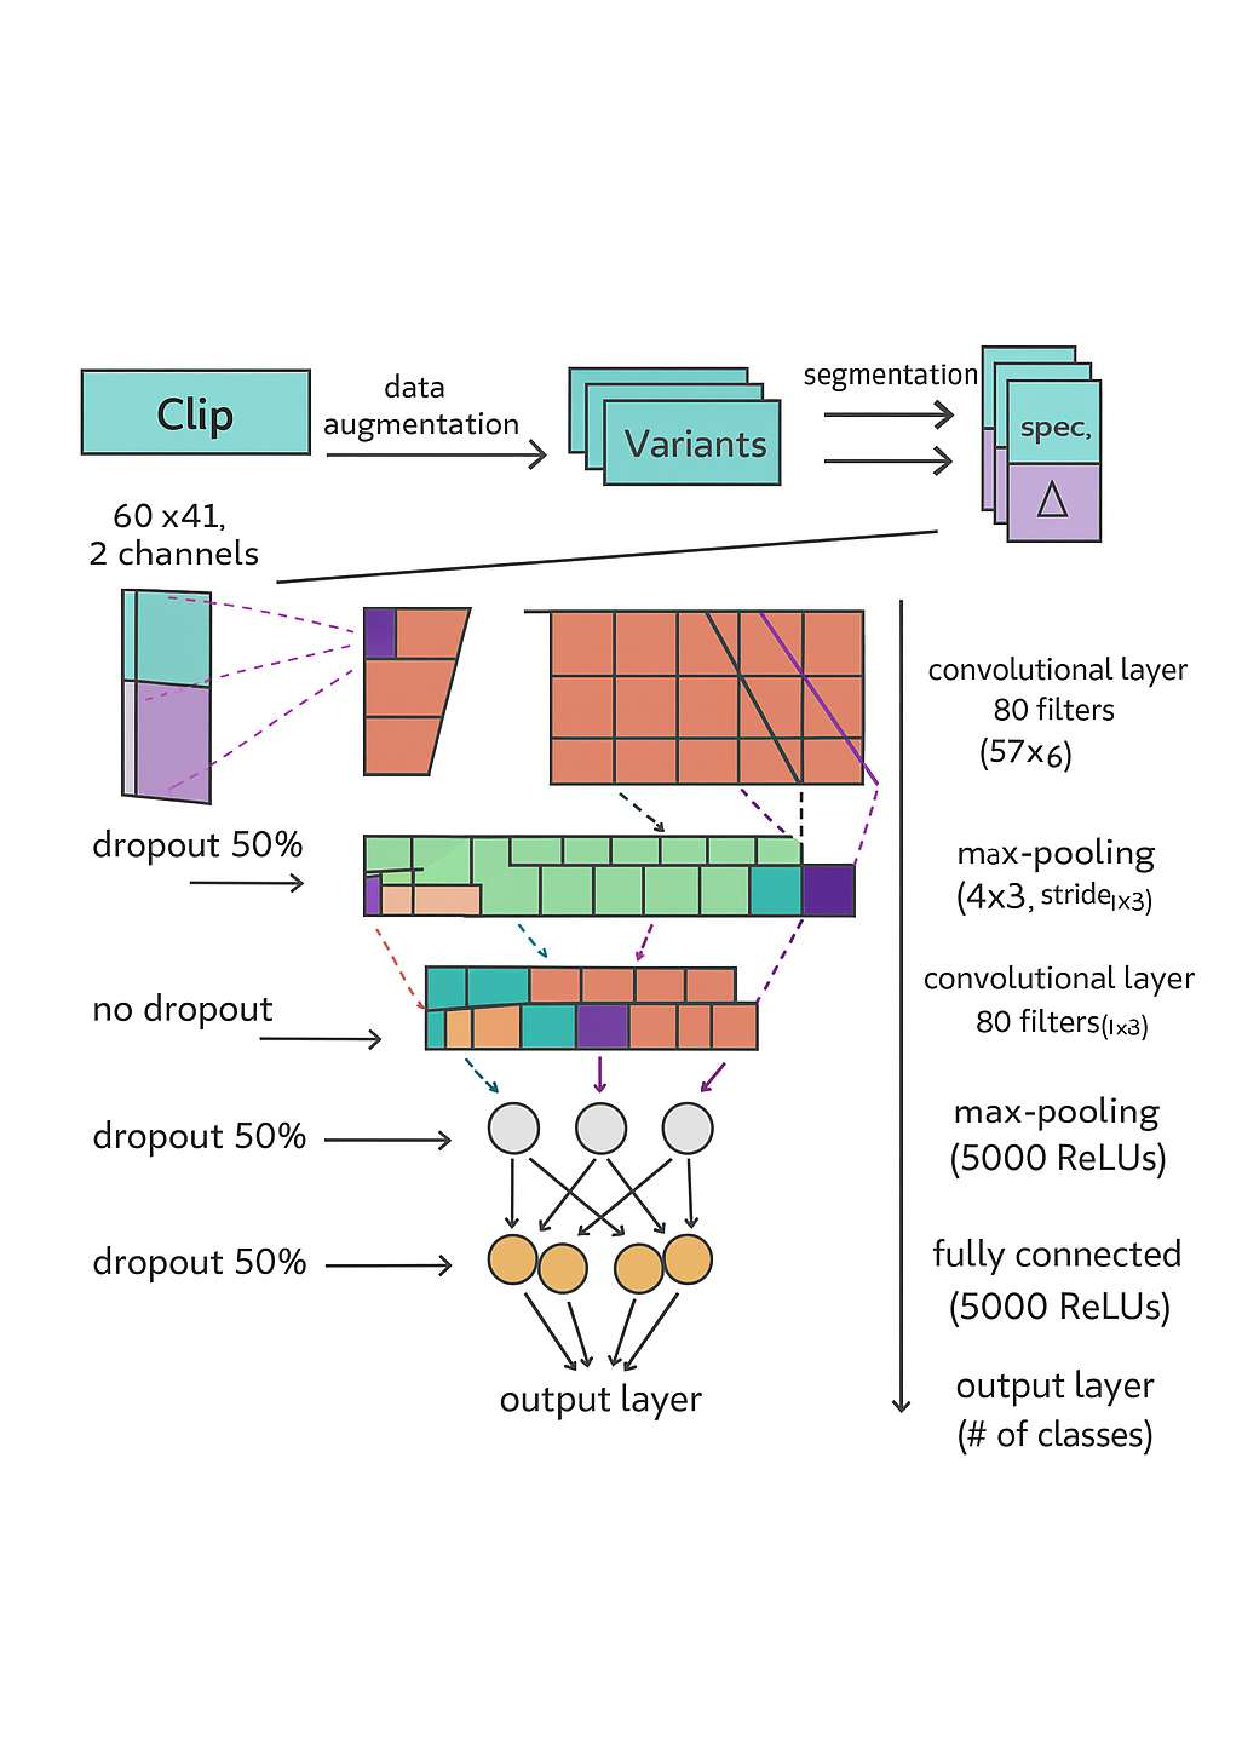
\includegraphics[width=0.55\linewidth]{arsitektur_piczak.pdf}
\caption{Arsitektur Piczak-CNN}
\end{figure}

\begin{enumerate}[leftmargin=1.25cm]
\item Conv1: 80 filter, kernel $57 \times 6$, aktivasi ReLU, diikuti max-pooling.
\item Conv2: 80 filter, kernel $1 \times 3$, aktivasi ReLU, diikuti max-pooling.
\item Fully connected: dua lapisan 5000 neuron.
\item Output: 5 neuron untuk klasifikasi lima kelas suara.
\end{enumerate}

Model pembanding adalah PANNs CNN14 yang di-fine-tune pada dataset identik. Komparasi diarahkan untuk mengevaluasi perbedaan performa dan efisiensi antara arsitektur kompak dan arsitektur besar pralatih.



\subsection{Training and Evaluation Protocol}
Konfigurasi pelatihan baseline menggunakan SGD, learning rate 0{,}002, momentum 0{,}9, batch size 32, maksimum 50 epoch, scheduler ReduceLROnPlateau, dan early stopping. Eksplorasi hyperparameter dilakukan pada 16 kombinasi:
\begin{itemize}[leftmargin=1.25cm]
\item Optimizer: SGD, Adam.
\item Dropout: 0{,}0; 0{,}1; 0{,}2; 0{,}3.
\item Augmentasi: aktif, nonaktif.
\end{itemize}

Metrik evaluasi meliputi accuracy, precision, recall, dan F1-score. Untuk agregasi lintas fold digunakan rerata:
\begin{equation}
\bar{x}=\frac{1}{K}\sum_{i=1}^{K}x_i,\quad K=5
\end{equation}

\subsection{Experimental Scenario and Fairness Control}
Agar perbandingan antarskenario tetap adil, seluruh eksperimen mengikuti protokol yang sama pada aspek-aspek berikut:
\begin{enumerate}[leftmargin=1.25cm]
\item Struktur pembagian fold tetap (seed 42 dan stratified split yang sama untuk semua skenario).
\item Durasi pelatihan maksimum, ukuran batch, dan kriteria early stopping tidak diubah.
\item Pre-processing utama (log-Mel 60 bin, segmentasi 41 frame, dan fitur delta) dijaga konstan.
\item Perbedaan antar eksperimen hanya berasal dari faktor yang diuji: optimizer, dropout, dan status augmentasi.
\end{enumerate}

Pendekatan ini penting untuk mengurangi bias eksperimen. Dengan kontrol tersebut, perubahan metrik dapat diatribusikan secara lebih kuat kepada komponen yang sedang diuji, bukan akibat perubahan prosedur lain.

\subsection{Evaluation Metric Formulation}
Selain accuracy, evaluasi multiclass dilengkapi precision, recall, dan F1-score karena ketiga metrik ini memberikan gambaran ketepatan prediksi antar kelas yang lebih detail. Formulasi yang digunakan adalah:
\begin{equation}
\mathrm{Precision}=\frac{TP}{TP+FP}
\end{equation}
\begin{equation}
\mathrm{Recall}=\frac{TP}{TP+FN}
\end{equation}
\begin{equation}
\mathrm{F1}=2\cdot\frac{\mathrm{Precision}\cdot\mathrm{Recall}}{\mathrm{Precision}+\mathrm{Recall}}
\end{equation}

Untuk interpretasi praktis, nilai rata-rata antar fold digunakan sebagai indikator utama robustnes model. Metrik per fold tetap dilaporkan untuk melihat stabilitas performa pada partisi data yang berbeda.

\section{Result and Discussion}
\subsection{Hyperparameter Tuning Result}
Eksperimen menunjukkan pengaruh hyperparameter yang signifikan terhadap kinerja model. Tabel berikut merangkum seluruh kombinasi yang diuji.

\begin{table}[H]
\centering
\fontsize{8pt}{10pt}\selectfont
\caption{Hasil eksperimen pemilihan hyperparameter}
\begin{tabular}{cccccc}
\hline
No & Opt. & LR & Dropout & Aug. & Akurasi \\
\hline
0 & SGD & 0,002 & 0,5 & Ya & 0,598 \\
1 & SGD & 0,002 & 0,0 & Ya & 0,728 \\
2 & SGD & 0,002 & 0,0 & Tidak & 0,822 \\
3 & SGD & 0,002 & 0,1 & Ya & 0,772 \\
4 & SGD & 0,002 & 0,1 & Tidak & 0,822 \\
5 & SGD & 0,002 & 0,2 & Ya & 0,740 \\
6 & SGD & 0,002 & 0,2 & Tidak & 0,812 \\
7 & SGD & 0,002 & 0,3 & Ya & 0,726 \\
8 & SGD & 0,002 & 0,3 & Tidak & 0,818 \\
9 & Adam & 0,001 & 0,0 & Ya & 0,712 \\
10 & Adam & 0,001 & 0,0 & Tidak & 0,722 \\
11 & Adam & 0,001 & 0,1 & Ya & 0,702 \\
12 & Adam & 0,001 & 0,1 & Tidak & 0,770 \\
13 & Adam & 0,001 & 0,2 & Ya & 0,654 \\
14 & Adam & 0,001 & 0,2 & Tidak & 0,740 \\
15 & Adam & 0,001 & 0,3 & Ya & 0,680 \\
16 & Adam & 0,001 & 0,3 & Tidak & 0,578 \\
\hline
\end{tabular}
\end{table}

Tiga konfigurasi terbaik kemudian diverifikasi ulang tiga kali untuk menguji konsistensi.

\begin{table}[H]
\centering
\fontsize{8pt}{10pt}\selectfont
\caption{Verifikasi tiga konfigurasi terbaik}
\begin{tabular}{ccccc}
\hline
Dropout & Percobaan 1 & Percobaan 2 & Percobaan 3 & Rata-rata \\
\hline
0,0 & 0,822 & 0,812 & 0,836 & 0,823 \\
0,1 & 0,822 & 0,808 & 0,724 & 0,785 \\
0,3 & 0,818 & 0,804 & 0,810 & 0,811 \\
\hline
\end{tabular}
\end{table}

Konfigurasi optimal ditetapkan pada SGD, learning rate 0,002, dropout 0,0, dan tanpa augmentasi, dengan akurasi rata-rata 0,823 pada tahap verifikasi serta 0,836 pada evaluasi komparatif akhir.

\subsection{Detailed Reading of Hyperparameter Trend}
Jika hasil pada Tabel pemilihan hyperparameter ditelaah lebih rinci, terdapat pola yang konsisten pada hampir seluruh kombinasi: konfigurasi tanpa augmentasi memberikan akurasi lebih tinggi dibanding konfigurasi dengan augmentasi aktif pada nilai dropout yang sama. Misalnya, pada optimizer SGD dan dropout 0,0, akurasi naik dari 0,728 (augmentasi aktif) menjadi 0,822 (augmentasi nonaktif). Pola yang sama muncul pada dropout 0,1 (0,772 menjadi 0,822), dropout 0,2 (0,740 menjadi 0,812), dan dropout 0,3 (0,726 menjadi 0,818).

Pada optimizer Adam, kecenderungan serupa juga terlihat. Konfigurasi tanpa augmentasi umumnya lebih baik dibandingkan augmentasi aktif, meskipun nilainya tetap berada di bawah SGD. Hal ini memperkuat indikasi bahwa distribusi data sintetis hasil augmentasi pada eksperimen ini belum sepenuhnya selaras dengan karakter data validasi.

\begin{table}[H]
\centering
\fontsize{8pt}{10pt}\selectfont
\caption{Ringkasan selisih akurasi augmentasi aktif vs nonaktif}
\begin{tabular}{lcccc}
\hline
Optimizer & Dropout 0,0 & Dropout 0,1 & Dropout 0,2 & Dropout 0,3 \\
\hline
SGD (Nonaktif - Aktif) & +0,094 & +0,050 & +0,072 & +0,092 \\
Adam (Nonaktif - Aktif) & +0,010 & +0,068 & +0,086 & -0,102 \\
\hline
\end{tabular}
\end{table}

Tabel ringkasan tersebut memperlihatkan bahwa keuntungan mematikan augmentasi paling stabil pada optimizer SGD. Satu anomali pada Adam dropout 0,3 (selisih negatif) menguatkan kesimpulan bahwa interaksi antar-hyperparameter tidak linear dan perlu dibaca bersama konfigurasi optimizer.

\subsection{Training Stability Across Folds}
Selain nilai rata-rata, stabilitas antarfold diamati dari variasi metrik pada konfigurasi terbaik. Pada Piczak-CNN, akurasi per fold berada di rentang 0,76 sampai 0,90. Rentang ini menunjukkan model mampu mempertahankan performa pada variasi partisi data yang berbeda, walaupun tetap terdapat fluktuasi yang wajar pada dataset berukuran terbatas.

Pada model pembanding PANNs CNN14, rentang akurasi berada di 0,57 sampai 0,71. Selain rerata yang lebih rendah, rentang ini juga menunjukkan bahwa model besar belum memperoleh keuntungan yang konsisten pada domain data penelitian. Temuan ini mendukung argumen bahwa kesesuaian arsitektur terhadap domain data lebih menentukan daripada ukuran model semata.

\begin{table}[H]
\centering
\fontsize{8pt}{10pt}\selectfont
\caption{Ringkasan statistik sederhana metrik akurasi per fold}
\begin{tabular}{lccc}
\hline
Model & Minimum & Maksimum & Rentang \\
\hline
Piczak-CNN & 0,76 & 0,90 & 0,14 \\
PANNs CNN14 & 0,57 & 0,71 & 0,14 \\
\hline
\end{tabular}
\end{table}

Meskipun rentang keduanya sama pada data ini, titik pusat performa Piczak-CNN berada pada level yang jauh lebih tinggi. Artinya, fluktuasi yang terjadi masih berada pada zona performa yang lebih baik dibanding model pembanding.

\subsection{Ablation Study}
Studi ablasi dilakukan bertahap untuk menilai kontribusi komponen pelatihan:
\begin{enumerate}[leftmargin=1.25cm]
\item \textbf{Baseline}: dropout 0,5 dan augmentasi aktif menghasilkan 0,598.
\item \textbf{Variasi dropout}: menurunkan dropout ke 0,0 (augmentasi aktif) meningkatkan akurasi menjadi 0,728.
\item \textbf{Augmentasi nonaktif}: pada dropout 0,0 akurasi meningkat ke 0,822.
\item \textbf{Perbandingan optimizer}: SGD (0,822) lebih tinggi dari Adam (0,722) pada konfigurasi yang setara.
\end{enumerate}

Temuan ini menunjukkan bahwa regularisasi yang terlalu kuat tidak selalu sesuai untuk dataset terbatas. Selain itu, strategi augmentasi yang digunakan pada penelitian ini belum memberikan keuntungan performa pada distribusi data yang ada.

\begin{table}[H]
\centering
\fontsize{8pt}{10pt}\selectfont
\caption{Ringkasan empat skenario studi ablasi}
\begin{tabular}{p{3.7cm}p{6.2cm}c}
\hline
Skenario & Konfigurasi kunci & Akurasi \\
\hline
Baseline lengkap & SGD, lr 0,002, dropout 0,5, augmentasi aktif & 0,598 \\
Variasi dropout terbaik & SGD, lr 0,002, dropout 0,0, augmentasi aktif & 0,728 \\
Evaluasi augmentasi & SGD, lr 0,002, dropout 0,0, augmentasi nonaktif & 0,822 \\
Perbandingan optimizer & Adam, lr 0,001, dropout 0,0, augmentasi nonaktif & 0,722 \\
\hline
\end{tabular}
\end{table}

Kenaikan dari baseline ke konfigurasi terbaik sementara mencapai 0,224 poin akurasi absolut. Besarnya kenaikan ini menandakan bahwa konfigurasi pelatihan memiliki peran yang sangat dominan terhadap performa akhir, bahkan pada arsitektur yang sama.

\subsection{Comparison with PANNs CNN14}
Perbandingan per fold antara Piczak-CNN dan PANNs CNN14 disajikan sebagai berikut.

\begin{table}[H]
\centering
\fontsize{8pt}{10pt}\selectfont
\caption{Perbandingan Arsitektur Model Piczak-CNN dan PANNs CNN14}
\begin{tabular}{p{4.9cm}p{3.2cm}p{3.1cm}}
\hline
Aspek & Piczak-CNN & PANNs CNN14 \\
\hline
Jumlah blok konvolusi & 2 & 6 \\
Jumlah filter & 80 & 64--2048 \\
Ukuran kernel & $57\times6$, $1\times3$ & $3\times3$ \\
Pooling & Max pooling & Average pooling \\
Batch normalization & Tidak & Ya \\
Dropout rate & 0,0 & 0,2 (konvolusi), 0,5 (FC) \\
Jumlah unit FC & 5000 & 2048 \\
Pre-trained & Tidak & Ya (AudioSet) \\
Jumlah saluran masukan & 2 (log-Mel + delta) & 1 (log-Mel) \\
Optimizer & SGD & SGD \\
Learning rate & 0,002 & 0,002 \\
Jumlah kelas keluaran & 5 & 5 \\
\hline
\end{tabular}
\end{table}

\begin{table}[H]
\centering
\fontsize{8pt}{10pt}\selectfont
\caption{Perbandingan performa per fold}
\begin{tabular}{lcccccc}
\hline
 & \multicolumn{3}{c}{Piczak-CNN} & \multicolumn{3}{c}{PANNs CNN14} \\
Fold & Acc. & F1 & Prec. & Acc. & F1 & Prec. \\
\hline
1 & 0,87 & 0,8720 & 0,8757 & 0,57 & 0,5801 & 0,6069 \\
2 & 0,76 & 0,7186 & 0,8149 & 0,65 & 0,5979 & 0,6704 \\
3 & 0,90 & 0,8935 & 0,9002 & 0,71 & 0,6926 & 0,7263 \\
4 & 0,86 & 0,8569 & 0,8615 & 0,64 & 0,6336 & 0,6838 \\
5 & 0,79 & 0,7556 & 0,7942 & 0,63 & 0,6119 & 0,6641 \\
Rata-rata & 0,836 & 0,81932 & 0,8493 & 0,640 & 0,62322 & 0,6703 \\
\hline
\end{tabular}
\end{table}
Berdasarkan Tabel~10, perbandingan performa antara model Piczak-CNN dengan konfigurasi \textit{hyperparameter} terbaik (SGD, \textit{learning rate} 0{,}002, \textit{dropout rate} 0{,}0, tanpa augmentasi) dan model PANNs CNN14 yang di-\textit{fine-tune} pada dataset yang sama menunjukkan bahwa kedua model memiliki karakteristik performa yang berbeda. \par

Dari sisi efisiensi, Piczak-CNN memiliki ukuran 205 MB dengan 26,3 juta parameter, sedangkan PANNs CNN14 berukuran 319 MB dengan 80,7 juta parameter. Rasio akurasi per satu juta parameter adalah:
\begin{equation}
\frac{0{,}836}{26{,}3}=0{,}0318,\quad \frac{0{,}640}{80{,}7}=0{,}0079
\end{equation}

Rasio tersebut memperlihatkan efisiensi parameter Piczak-CNN sekitar empat kali lebih baik. Hasil ini menegaskan bahwa arsitektur kompak yang dioptimalkan secara domain-spesifik dapat lebih unggul dibanding model besar pada skenario data terbatas.

\begin{table}[H]
\centering
\fontsize{8pt}{10pt}\selectfont
\caption{Perbandingan efisiensi struktural model}
\begin{tabular}{lcc}
\hline
Aspek & Piczak-CNN & PANNs CNN14 \\
\hline
Ukuran model (MB) & 205 & 319 \\
Jumlah parameter (juta) & 26,3 & 80,7 \\
Akurasi rata-rata & 0,836 & 0,640 \\
Akurasi per juta parameter & 0,0318 & 0,0079 \\
\hline
\end{tabular}
\end{table}

Hasil pada tabel efisiensi menunjukkan bahwa keuntungan Piczak-CNN bukan hanya pada dimensi performa, tetapi juga pada rasio performa terhadap kompleksitas model. Ini merupakan temuan penting untuk aplikasi edge yang menuntut trade-off ketat antara akurasi dan sumber daya.

\subsection{Class-wise Error Interpretation}
Meskipun penelitian ini berfokus pada metrik agregat, pembacaan kesalahan klasifikasi menunjukkan bahwa kelas dengan karakteristik spektral transien (misalnya pecahan kaca) cenderung sensitif terhadap variasi derau latar. Sebaliknya, kelas dengan pola harmonik yang lebih persisten (misalnya sirene) relatif lebih mudah dipelajari model. Pola ini sejalan dengan sifat representasi log-Mel dan fitur delta yang menonjolkan transisi energi terhadap waktu.

Kebingungan antarkelas paling mungkin terjadi pada pasangan kelas yang memiliki irisan energi frekuensi menengah dan envelope temporal yang serupa, seperti klakson mobil dan klakson motor. Dalam konteks aplikasi keselamatan, kebingungan antarkelas ini masih lebih dapat ditoleransi dibanding kegagalan mendeteksi sinyal bahaya sama sekali, karena keduanya tetap termasuk kategori peringatan lalu lintas.

\begin{table}[H]
\centering
\fontsize{8pt}{10pt}\selectfont
\caption{Ilustrasi matriks kebingungan multiclass (struktur evaluasi)}
\begin{tabular}{lccccc}
\hline
Prediksi / Aktual & Sirene & Klk. Mobil & Klk. Motor & Kaca Pecah & Tng. Bayi \\
\hline
Sirene & TP & FP & FP & FP & FP \\
Klk. Mobil & FP & TP & FP & FP & FP \\
Klk. Motor & FP & FP & TP & FP & FP \\
Kaca Pecah & FP & FP & FP & TP & FP \\
Tng. Bayi & FP & FP & FP & FP & TP \\
\hline
\end{tabular}
\end{table}

Struktur pada tabel tersebut digunakan untuk menganalisis distribusi kesalahan secara sistematis pada setiap fold. Dengan pendekatan ini, analisis tidak hanya berhenti pada nilai akurasi global, tetapi juga mempertimbangkan arah kesalahan prediksi antarkelas.

\subsection{Interpretation and Practical Implication}
Temuan penelitian memiliki implikasi praktis penting. Pertama, kesesuaian domain data terbukti sangat berpengaruh terhadap performa model. Kedua, kombinasi regularisasi perlu disesuaikan dengan ukuran dan karakter data; konfigurasi yang efektif pada dataset besar belum tentu cocok pada dataset terbatas. Ketiga, keunggulan efisiensi Piczak-CNN membuka peluang implementasi pada perangkat edge untuk sistem peringatan real-time.

Meski demikian, penelitian ini masih bersifat evaluasi offline. Pengukuran latensi inferensi end-to-end pada perangkat target dan uji lapangan masih diperlukan untuk menilai kesiapan implementasi produksi.

\subsection{Deployment Perspective for Assistive System}
Dalam skenario implementasi, model dapat dipasang pada pipeline inferensi sederhana: akuisisi audio kontinu, framing jendela pendek, ekstraksi fitur log-Mel + delta, inferensi kelas, lalu pemetaan hasil ke notifikasi visual/haptik pada perangkat pengguna. Karena ukuran model relatif kecil, strategi deployment ini lebih realistis untuk perangkat mobile dibanding model yang jauh lebih besar.

Dari sisi pengalaman pengguna, keluaran sistem sebaiknya tidak langsung ditampilkan sebagai label mentah, tetapi dikelompokkan ke prioritas tindakan, misalnya: \textit{peringatan lalu lintas} (klakson/sirene), \textit{peringatan keamanan rumah} (pecahan kaca), dan \textit{peringatan domestik} (tangisan bayi). Pendekatan ini berpotensi menurunkan beban kognitif pengguna dan mempercepat respons pada situasi kritis.

Dalam implementasi lebih lanjut, sistem dapat dilengkapi mekanisme smoothing prediksi berbasis jendela waktu singkat agar notifikasi lebih stabil dan tidak mudah berfluktuasi karena noise sesaat. Selain itu, ambang keputusan (decision threshold) dapat diatur berbeda untuk kelas berisiko tinggi seperti sirene, sehingga sensitivitas deteksi pada sinyal kritis dapat ditingkatkan.

\subsection{Extended Discussion}
Secara metodologis, penelitian ini menunjukkan bahwa pengoptimalan komponen pelatihan pada model kompak mampu menghasilkan lompatan performa yang signifikan. Dari baseline 0,598 ke konfigurasi optimal 0,836, terdapat peningkatan absolut sebesar 0,238. Nilai ini mengindikasikan bahwa strategi tuning yang sistematis dapat memberikan dampak besar tanpa harus mengganti arsitektur ke model yang lebih berat.

Dari perspektif rekayasa sistem, hasil ini memperkuat prinsip bahwa pemilihan model harus mempertimbangkan konteks deployment. Pada kondisi perangkat terbatas, model yang lebih kecil namun teroptimasi sering lebih praktis dibanding model besar yang memerlukan sumber daya tinggi. Prinsip ini sejalan dengan kebutuhan sistem assistive technology yang menuntut respons cepat, konsumsi daya rendah, dan reliabilitas di lingkungan nyata.

\subsection{Use-case Analysis and Operational Risk}
Untuk skenario pengguna akhir, sistem klasifikasi suara ini dapat dioperasikan sebagai modul pemantauan pasif yang berjalan di latar belakang perangkat mobile. Ketika model mendeteksi kelas suara tertentu dengan tingkat keyakinan di atas ambang yang ditentukan, sistem memicu notifikasi visual atau getaran. Pola respons semacam ini relevan untuk pengguna dengan gangguan pendengaran karena mengubah sinyal auditif kritis menjadi sinyal yang dapat diindera secara langsung.

Analisis operasional menunjukkan bahwa kesalahan model memiliki tingkat konsekuensi yang berbeda. False negative pada kelas sirene, misalnya, berpotensi lebih berisiko dibanding false negative pada kelas lain karena berkaitan langsung dengan kendaraan prioritas di jalan. Oleh karena itu, desain deployment sebaiknya mempertimbangkan kebijakan berbasis kelas (class-aware policy), misalnya ambang deteksi yang lebih sensitif untuk suara berisiko tinggi.

Di sisi lain, false positive berulang juga dapat menurunkan kepercayaan pengguna terhadap sistem. Untuk mengurangi masalah ini, dapat diterapkan strategi verifikasi temporal, yaitu notifikasi baru diberikan jika prediksi konsisten dalam beberapa jendela waktu berturut-turut. Strategi ini menyeimbangkan kebutuhan sensitivitas dan spesifisitas agar sistem lebih nyaman digunakan pada kondisi nyata yang bising.

\begin{table}[H]
\centering
\fontsize{8pt}{10pt}\selectfont
\caption{Contoh prioritas risiko operasional per kelas suara}
\begin{tabular}{p{3.3cm}p{3.1cm}p{3.8cm}}
\hline
Kelas suara & Tingkat prioritas & Rekomendasi respons sistem \\
\hline
Sirene & Tinggi & Notifikasi segera dengan getaran kuat dan tampilan visual kontras \\
Klakson mobil/motor & Tinggi & Notifikasi cepat, dapat digabung dalam kategori peringatan lalu lintas \\
Pecahan kaca & Menengah-tinggi & Notifikasi keamanan dengan penanda lokasi/waktu kejadian \\
Tangisan bayi & Menengah & Notifikasi domestik dengan mode pengulangan adaptif \\
\hline
\end{tabular}
\end{table}

Pendekatan berbasis prioritas seperti pada tabel di atas memperkuat nilai praktis model karena keluaran klasifikasi diterjemahkan menjadi aksi yang bermakna bagi pengguna, bukan hanya label prediksi.

\subsection{Roadmap for Future Experimental Extension}
Sebagai kelanjutan penelitian, terdapat tiga arah eksperimen yang paling potensial. Pertama, memperluas data dengan variasi noise lingkungan nyata (jalan raya, pasar, terminal, ruang tertutup) untuk menguji robustnes domain shift. Kedua, melakukan uji latensi end-to-end pada perangkat target untuk memastikan kesesuaian kebutuhan real-time. Ketiga, mengevaluasi skema threshold adaptif per kelas agar sistem dapat menyeimbangkan sensitivitas deteksi suara berisiko tinggi dan stabilitas notifikasi jangka panjang.

Jika ketiga arah ini dilaksanakan, maka kontribusi penelitian tidak hanya berhenti pada performa klasifikasi offline, tetapi dapat bergerak menuju prototipe assistive system yang lebih siap diimplementasikan.

\subsection{Threats to Validity}
Beberapa keterbatasan penelitian yang perlu dicatat adalah sebagai berikut. Pertama, ukuran dataset masih terbatas pada 500 sampel sehingga variasi akustik dunia nyata belum sepenuhnya terwakili. Kedua, seluruh eksperimen dibatasi pada lima kelas suara prioritas; ketika kelas diperluas, performa model dapat berubah. Ketiga, evaluasi dilakukan secara offline dengan cross-validation, sehingga performa pada aliran audio kontinu real-time belum diukur langsung.

Meskipun demikian, rancangan eksperimen yang konsisten antarskenario, penggunaan pembagian fold yang tetap, serta laporan metrik komprehensif membantu menjaga validitas internal penelitian.

\section{Supplementary Experimental Notes}
Bagian ini merangkum catatan eksperimen tambahan yang digunakan untuk meningkatkan keterlacakan proses penelitian dari tahap data hingga evaluasi. Walaupun tidak mengubah kesimpulan utama, rincian ini membantu pembaca memahami keputusan teknis yang diambil selama pengembangan model.

\subsection{Fold Construction and Reproducibility Note}
Setiap fold dibangun menggunakan stratified split dengan seed tetap agar distribusi kelas antar fold konsisten. Strategi ini menghindari dominasi kelas tertentu pada salah satu fold yang dapat menyebabkan estimasi performa menjadi bias. Dalam praktiknya, konsistensi pembagian data menjadi faktor penting karena perubahan fold dapat menghasilkan deviasi metrik yang tidak merepresentasikan perubahan kualitas model sebenarnya.

Untuk menjaga reprodusibilitas, seluruh skenario pengujian menggunakan indeks fold yang sama. Dengan cara ini, perbandingan antar-konfigurasi benar-benar mengukur dampak perubahan hyperparameter, bukan dampak perbedaan data validasi.

\subsection{Operational Observation per Fold}
Pengamatan selama eksperimen menunjukkan bahwa fold dengan akurasi tertinggi umumnya memiliki separabilitas kelas yang lebih jelas pada domain spektrogram, terutama untuk kelas sirene dan pecahan kaca. Sementara itu, fold dengan akurasi lebih rendah cenderung memuat lebih banyak contoh dengan karakteristik akustik tumpang tindih pada kelas klakson mobil dan klakson motor.

Secara praktis, observasi ini memperkuat pentingnya pengayaan data pada pasangan kelas yang beririsan. Peningkatan kualitas dataset pada area tersebut diperkirakan memberi dampak yang lebih besar daripada sekadar memperdalam arsitektur model.

\begin{table}[H]
\centering
\fontsize{8pt}{10pt}\selectfont
\caption{Ringkasan observasi karakteristik kelas pada evaluasi}
\begin{tabular}{p{3.1cm}p{3.4cm}p{4.0cm}}
\hline
Kelas & Ciri umum pada spektrogram & Catatan evaluasi \\
\hline
Sirene & Pola harmonik berulang dan stabil & Relatif mudah dikenali di sebagian besar fold \\
Klakson mobil & Energi menengah-tinggi dengan pola impulsif & Beririsan dengan klakson motor pada beberapa sampel \\
Klakson motor & Pola impulsif dengan variasi lebih tinggi & Kebingungan kelas meningkat pada data bising \\
Pecahan kaca & Transien tajam berdurasi singkat & Sensitif terhadap noise latar yang mendadak \\
Tangisan bayi & Variasi harmonik dan envelope temporal dinamis & Umumnya terdeteksi baik, namun dapat overlap dengan noise rumah tangga \\
\hline
\end{tabular}
\end{table}

\subsection{Implication for Further Benchmarking}
Untuk benchmark lanjutan, penelitian dapat menambahkan dua jalur evaluasi. Jalur pertama adalah evaluasi robustnes terhadap noise terkontrol dengan level SNR bertingkat agar ketahanan model dapat diukur kuantitatif. Jalur kedua adalah evaluasi berbasis skenario penggunaan, misalnya simulasi perjalanan di jalan raya dan simulasi lingkungan domestik.

Dengan dua jalur tersebut, capaian model tidak hanya dinilai dari metrik klasifikasi standar, tetapi juga dari kesesuaian terhadap kebutuhan operasional pengguna akhir. Pendekatan ini sejalan dengan tujuan penelitian yang berorientasi pada sistem peringatan asistif.

\section{Conclusion and Suggestion}
Penelitian ini menunjukkan bahwa optimasi Piczak-CNN berbasis representasi log-Mel spectrogram efektif untuk klasifikasi lima suara peringatan keselamatan. Konfigurasi terbaik (SGD, learning rate 0{,}002, dropout 0{,}0, tanpa augmentasi) menghasilkan akurasi rata-rata 83{,}6\%, F1-score 0{,}81932, dan presisi 0{,}8493. Dibandingkan PANNs CNN14, model usulan tidak hanya lebih akurat pada dataset yang sama, tetapi juga lebih efisien secara komputasional.

Untuk pengembangan selanjutnya, disarankan memperluas dataset dengan variasi kondisi akustik nyata, menguji teknik augmentasi yang lebih adaptif, menambahkan evaluasi latensi dan konsumsi daya pada perangkat edge, serta mengintegrasikan keluaran model ke antarmuka multimodal (visual atau haptik) untuk meningkatkan manfaat pada pengguna dengan gangguan pendengaran.

\section*{Acknowledgement}
Penulis mengucapkan terima kasih kepada dosen pembimbing, dosen penguji, serta Program Studi Teknik Informatika Institut Teknologi Sumatera atas dukungan akademik selama pelaksanaan penelitian ini.

\section*{Declarations}
AUTHOR CONTRIBUTION\\
Penulis tunggal bertanggung jawab atas konseptualisasi, pengumpulan data, implementasi model, evaluasi, analisis hasil, serta penulisan naskah.\\

FUNDING STATEMENT\\
Penelitian ini tidak menerima pendanaan khusus dari lembaga pemerintah, komersial, maupun nirlaba.\\

COMPETING INTEREST\\
Penulis menyatakan tidak terdapat konflik kepentingan dalam penelitian ini.

\printbibliography

\end{document}
